\section{Experiments}\label{sec:experiments}
In this section, we detail the experiments conducted to evaluate the performance of each component within the MOC pipeline.
Our initial step was to establish a baseline using the replica of the MOC pipeline described in Section~\ref{sec:methodology}.
This baseline serves as a reference point for comparison and assessment of experimental results.

The experiments are structured as follows:

\begin{enumerate}
    \item Evaluating the necessity of automated outlier removal in the PLS1-SM component by comparing performance with and without this process.
    \item Investigating the effect of fixed threshold values in the outlier removal process of PLS1-SM, maintaining these thresholds from the second iteration onwards.
    \item Assessing the impact of the Median Absolute Deviation (MAD) method for outlier removal in the Independent Component Analysis (ICA) phase.
    \item Determining the effect on ICA performance when utilizing datasets from five locations compared to a single dataset.
    \item Comparing the performance of PLS1-SM and ICA models against alternative models, such as XGBoost and Artificial Neural Networks (ANN).
\end{enumerate}

These experiments were selected to explore the significance of the outlier removal process, the optimization of threshold values, and the comparative effectiveness of different modeling approaches within the MOC pipeline.
The first experiment focuses on the automated outlier removal process in PLS1-SM, examining its necessity by comparing outcomes with and without this step.
The second experiment looks at the implications of using fixed threshold values for outlier removal in PLS1-SM, opting for a conservative approach by not updating these values after each iteration.
In the third experiment, we apply the MAD method for outlier removal in ICA, comparing its effectiveness against the baseline.
The fourth experiment evaluates ICA's performance using aggregated datasets from multiple locations, aiming to understand the balance between representativeness and information loss.
The final experiment extends the analysis to include comparisons with other models, providing a broader perspective on the MOC pipeline's performance.


This experimental approach allows for assessment of the MOC pipeline's components, offering insights into their individual and collective impacts on the system's overall performance.


Given our replication of the MOC pipeline, we are now in a position to conduct experiments to evaluate the performance of each of the components in the pipeline.
We start by describing the baseline we have established, which serves as basis for comparison with the original MOC pipeline and for assessing experimental results.
Then, we describe the experiments we have conducted to evaluate the performance of each of the components in the pipeline.

To evaluate the performance of each of the components in the pipeline, we have conducted the following series of experiments.

\begin{enumerate}
	\item\label{enum:experiment1} No outlier removal for PLS1-SM to evaluate the significance of our automated outlier removal process and whether outlier removal is necessary.
	\item\label{enum:experiment2} Maintain the threshold values from the second iteration of the outlier removal in the PLS1-SM training process to see if a more or less conservative approach is advantageous.
	\item\label{enum:experiment3} MAD for ICA to evaluate the significance of the outlier removal step in the ICA phase.
	\item\label{enum:experiment4} Evaluating the impact on ICA model performance when using all five location datasets versus just one.
	\item\label{enum:experiment5} Other models to compare the performance of the PLS1-SM and ICA models to other models.
	% \item PLS outlier removal on ICA (?) instead of MAD.
\end{enumerate}

\noindent
We have chosen these experiments based on the following reasons.
For Experiment~\ref{enum:experiment1}, we are interested in evaluating the significance of our automated outlier removal process due to its differences from the original manual process.
Additionally, we are interested in examining whether outlier removal is necessary for the PLS1-SM phase by comparing the results with and without outlier removal.

For Experiment~\ref{enum:experiment2}, we want to evaluate the significance of the threshold values used in the outlier removal process by maintaining the threshold values from the second iteration of the outlier removal in the PLS1-SM training process.
This is a more conservative than always updating the threshold values after each iteration.

For Experiment~\ref{enum:experiment3}, we implement our best guess of the original authors' outlier removal process for the ICA phase, which is based on the Median Absolute Deviation (MAD).
Then, we compare the results with and without MAD to evaluate the significance of the outlier removal step in the ICA phase.

For Experiment~\ref{enum:experiment4}, we perform ICA using all five location datasets by averaging the results from location into a single dataset.
By doing this, we will either obtain a more representative dataset for the sample, or we will end up losing information by averaging the results.

For Experiment~\ref{enum:experiment5}, we want to compare the performance of the MOC model with other models.
Specifically, we train an XGBoost model and an ANN model for comparison.

\subsection{Replication of the MOC Pipeline}\label{sec:replica_moc}
We present the baseline RMSEs of the original and our replicas of the PLS1-SM, ICA, and MOC models in Table~\ref{tab:results_rmses}.
Figure~\ref{fig:rmse_histograms} illustrates the distribution of the RMSEs of the original and our replicas of the PLS1-SM, ICA, and MOC models as a grouped histogram.
The results show that the RMSEs of our replicas of the PLS1-SM, ICA and MOC models are similar to the original models.
However, the are some notable differences --- in some cases, our replicas outperform the original models, while in other cases, the original models outperform our replicas.
These differences can be attributed to a number of factors.

Firstly, the original models were trained on two datasets, one acquired at a 1600mm standoff distance and one acquired at a 3000mm standoff distance.
We have only used the 1600mm dataset for our replicas since we do not have access to the 3000mm dataset.
As mentioned in Section~\ref{sec:outlier_removal}, we also chose chose to automate the outlier removal process for the PLS1-SM phase, whereas the original authors performed this manually.
Moreover, we chose to exclude the outlier removal step during the ICA phase to avoid introducing unsubstantiated assumptions, as described in Section~\ref{sec:ica_data_preprocessing}.
In Section~\ref{sec:ica_data_preprocessing}, we clarified that unlike the original authors who utilized all five location datasets, our analysis was limited to a single dataset per sample due to the absence of details on their integration.
For training the PLS models, \citet{andersonImprovedAccuracyQuantitative2017} methodically organized their training and test sets by sorting samples based on the major oxide, sequentially assigning them to folds, removing outliers, and deliberately including extreme compositions in the training folds to enhance the model's ability to handle a broad range of elemental variations.
Since we lack the domain expertise to replicate this process, we instead randomly split the dataset into training and test sets without any further curation using a 80/20 split.
Additionally, without going into speculations, it is possible that some of the differences are due to implementation details, such as the use of different programming languages and libraries.
Lastly, it is worth noting that RMSE is simply a statistical measure of the differences between the original and predicted values, and does not necessarily reflect the true accuracy of the models on unseen data from Mars, and so the results should be interpreted with this in mind.

\begin{table*}[h]
\centering
\begin{tabular*}{\textwidth}{@{\extracolsep{\fill}}lllllll}
\hline
Element    & PLS1-SM (original) & PLS1-SM (replica) & ICA (original) & ICA (replica) & MOC (original) & MOC (replica) \\
\hline
\ce{SiO2}  & 4.33               & 5.81              & 8.31           & 10.68         & 5.30           & 7.29 \\
\ce{TiO2}  & 0.94               & 0.47              & 1.44           & 0.63          & 1.03           & 0.49 \\
\ce{Al2O3} & 2.85               & 1.94              & 4.77           & 5.55          & 3.47           & 2.39 \\
\ce{FeO_T} & 2.01               & 4.35              & 5.17           & 8.30          & 2.31           & 5.21 \\
\ce{MgO}   & 1.06               & 1.17              & 4.08           & 2.90          & 2.21           & 1.67 \\
\ce{CaO}   & 2.65               & 1.43              & 3.07           & 3.52          & 2.72           & 1.81 \\
\ce{Na2O}  & 0.62               & 0.66              & 2.29           & 1.72          & 0.62           & 1.10 \\
\ce{K2O}   & 0.72               & 0.72              & 0.98           & 1.37          & 0.82           & 1.09 \\
\hline
\end{tabular*}
\caption{RMSE of the original and our replicas of the PLS1-SM, ICA, and MOC models.}
\label{tab:results_rmses}
\end{table*}

\begin{figure*}[b]
	\centering
	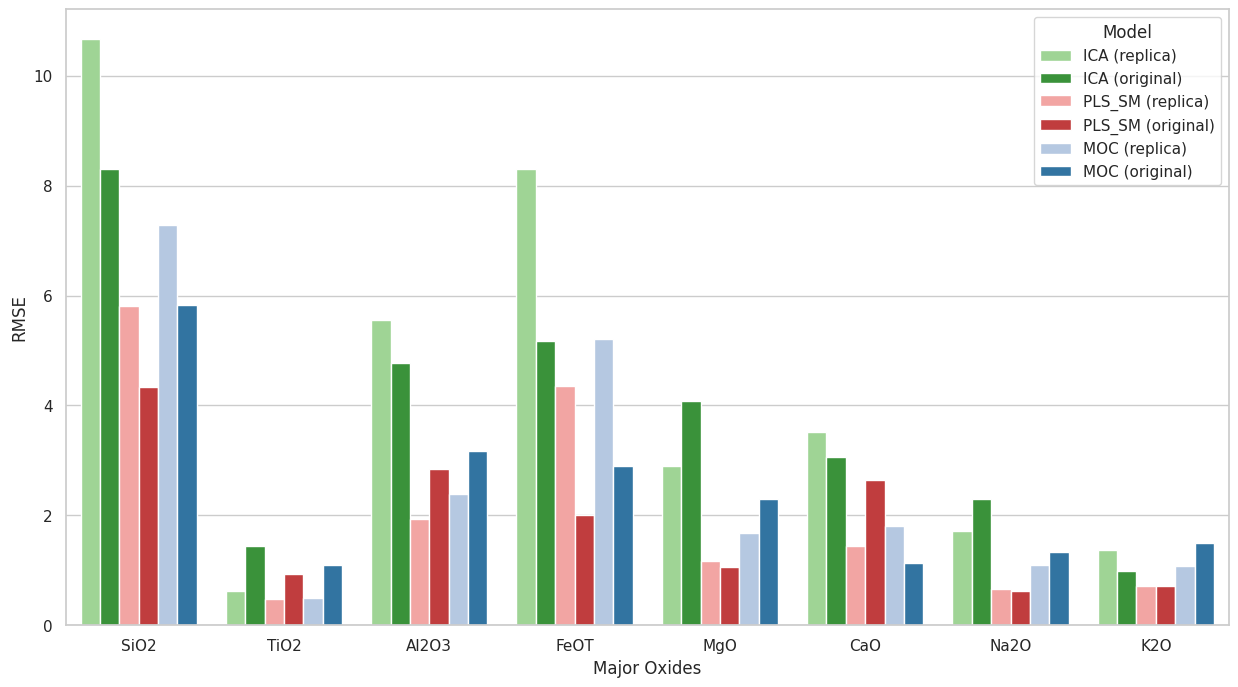
\includegraphics[width=0.85\textwidth]{images/rmse_historgram.png}
	\caption{Grouped histogram of the RMSEs of the original and our replicas of the PLS1-SM, ICA, and MOC models.}
	\label{fig:rmse_histograms}
\end{figure*}

To evaluate the statistical significance of the differences between the original and our replicated models (PLS1-SM, ICA, and MOC), we applied three statistical tests: Student's t-test, Welch's t-test, and the Wilcoxon signed-rank test.
Our null hypothesis (H$_0$) posits that there is no significant difference in the performance of the original and replicated models.
The alternative hypothesis (H$_1$) contends that a significant difference does exist.
We set our significance level $\alpha$ at 0.05, meaning we would require a p-value less than 0.05 to reject the null hypothesis in favor of the alternative.
The p-values obtained from our tests are presented in Table~\ref{tab:results_ttests}. With all p-values exceeding the $\alpha$ level of 0.05, there is insufficient statistical evidence to reject the null hypothesis.
Therefore, we retain the null hypothesis, suggesting that the differences between the original and replicated models are not statistically significant.
The p-values across all tests and models imply that the performances of the original and replicated models are statistically indistinguishable from each other.
This congruence suggests that our replicated models are comparable to the original ones in terms of their statistical characteristics.

\begin{table}[h]
\centering
\begin{tabular}{llll}
\hline
p-value    & Student's & Welch's & Wilcoxon \\
\hline
PLS1-SM    & 67.71\% & 84.04\% & 73.53\% \\
ICA        & 32.38\% & 71.38\% & 64.06\% \\
MOC        & 54.69\% & 75.45\% & 100.00\% \\
\hline
\end{tabular}
\caption{p-values of the Student's t-test, Welch's t-test, and Wilcoxon signed-rank test for the RMSEs between the original and our replicas of the PLS1-SM, ICA, and MOC models, respectively.}
\label{tab:results_ttests}
\end{table}

\subsection{Experiment: Outlier Removal}\label{sec:experiment_outlier_removal}
% TODO: Add results and discussion.

The original PLS1-SM identified outliers manually by inspecting the leverage and spectral residuals plots.
We have instead chosen to automate this based on the reasons described in Section~\ref{sec:methodology_outlier_removal}.
It would therefore be intriguing to examine the impact on the pipeline's performance when this process is adjusted.
Firstly, examining the performance implications of completely omitting outlier removal would be worthwhile.
This experiment is justified given the substantial efforts dedicated to developing the ChemCam calibration dataset as mentioned in Section~\ref{sec:ica_data_preprocessing}, which implies a minimal presence of significant outliers.
Secondly, maintaining the threshold values from the second iteration of the outlier removal in the PLS1-SM training process would lead to a more conservative outlier removal process where fewer samples are removed.
The reason for doing so is that we do not know the basis for the original author's manual outlier removal process, and it is possible that they were more conservative than our automated process.
Consequently, a more conservative approach could potentially align our replica of the pipeline more closely with the original.

In the ICA phase, the original authors employed the Median Absolute Deviation (MAD) for outlier removal, yet the detailed methodology of their approach was not fully delineated.
Consequently, in our version of the pipeline, we chose to exclude the outlier removal step during the ICA phase to avoid introducing unsubstantiated assumptions, as described in Section~\ref{sec:ica_data_preprocessing}.
This decision allows us to evaluate the intrinsic effectiveness of the ICA phase without the influence of outlier removal.
Introducing outlier removal using MAD in our replication of the pipeline presents an opportunity to assess its impact on the pipeline's efficacy.
By comparing the results with and without MAD, we can quantitatively measure the utility of this step.
Such an experiment is crucial for understanding whether MAD significantly contributes to reducing noise and improving data quality, thereby enhancing the overall performance of the machine learning pipeline.
This experiment would also offer insights into the robustness of the ICA phase against outliers, providing a more comprehensive understanding of the pipeline's capabilities and limitations.

\subsection{Experiment: Other Models}\label{sec:experiment_other_models}
\citet{cleggRecalibrationMarsScience2017} have only compared their new approach with the original method presented by \citet{wiensPreFlight3}, and have not conducted experiments using alternative methods to establish the superiority of their chosen approach.
Therefore, we decided to compare the performance of the PLS1-SM and ICA models to other models.
The objective is to evaluate two distinct scenarios.
In the first scenario, we aim to conduct a direct comparison between the MOC model and an alternative model. The second scenario revolves around substituting either PLS or ICA with a different model and then calculating a weighted average.
We have decided to conduct the experiments using the following models:

\begin{itemize}
	\item \textbf{XGBoost}, a gradient boosting algorithm, \cite{chen_xgboost_2016}.
	\item \textbf{ANN}, a neural network model, \cite{scikit-learn}.
\end{itemize}

% TODO: Argue why we chose these models (ref SuperCam paper).
% TODO: Add results and discussion.